% !TeX encoding = UTF-8
% !TeX program  = pdflatex

\documentclass[xcolor={svgnames,table},10pt,fleqn]{beamer}
\usepackage{stb-beamer-a}

%---- AMS math ---------------------------------------------------------
\usepackage{amsmath,amsthm}

%---- Fonts ------------------------------------------------------------
\usefonttheme{professionalfonts}
\usepackage[T1]{fontenc}
\usepackage{textcomp}
\usepackage[default,medium,scaled=1.0]{raleway}
\usepackage[scaled=0.80]{arevmath}

%---- Packages ---------------------------------------------------------
\usepackage{tikz}
\usepackage{booktabs}
\cmidrulewidth=\heavyrulewidth


%---- Title page -------------------------------------------------------
\title[\emph{Ergo}]{\emph{Ergo}}
\subtitle{A Gesture-Based Computer Interaction Device}

\author{Boyd Kane, Supervisor: Dr. Trienko Grobler}
\institute{Computer Science Division,\\
           Stellenbosch University}

\subject{Master's in Computer Science}
\date{February 2024}

\def\titlefig{{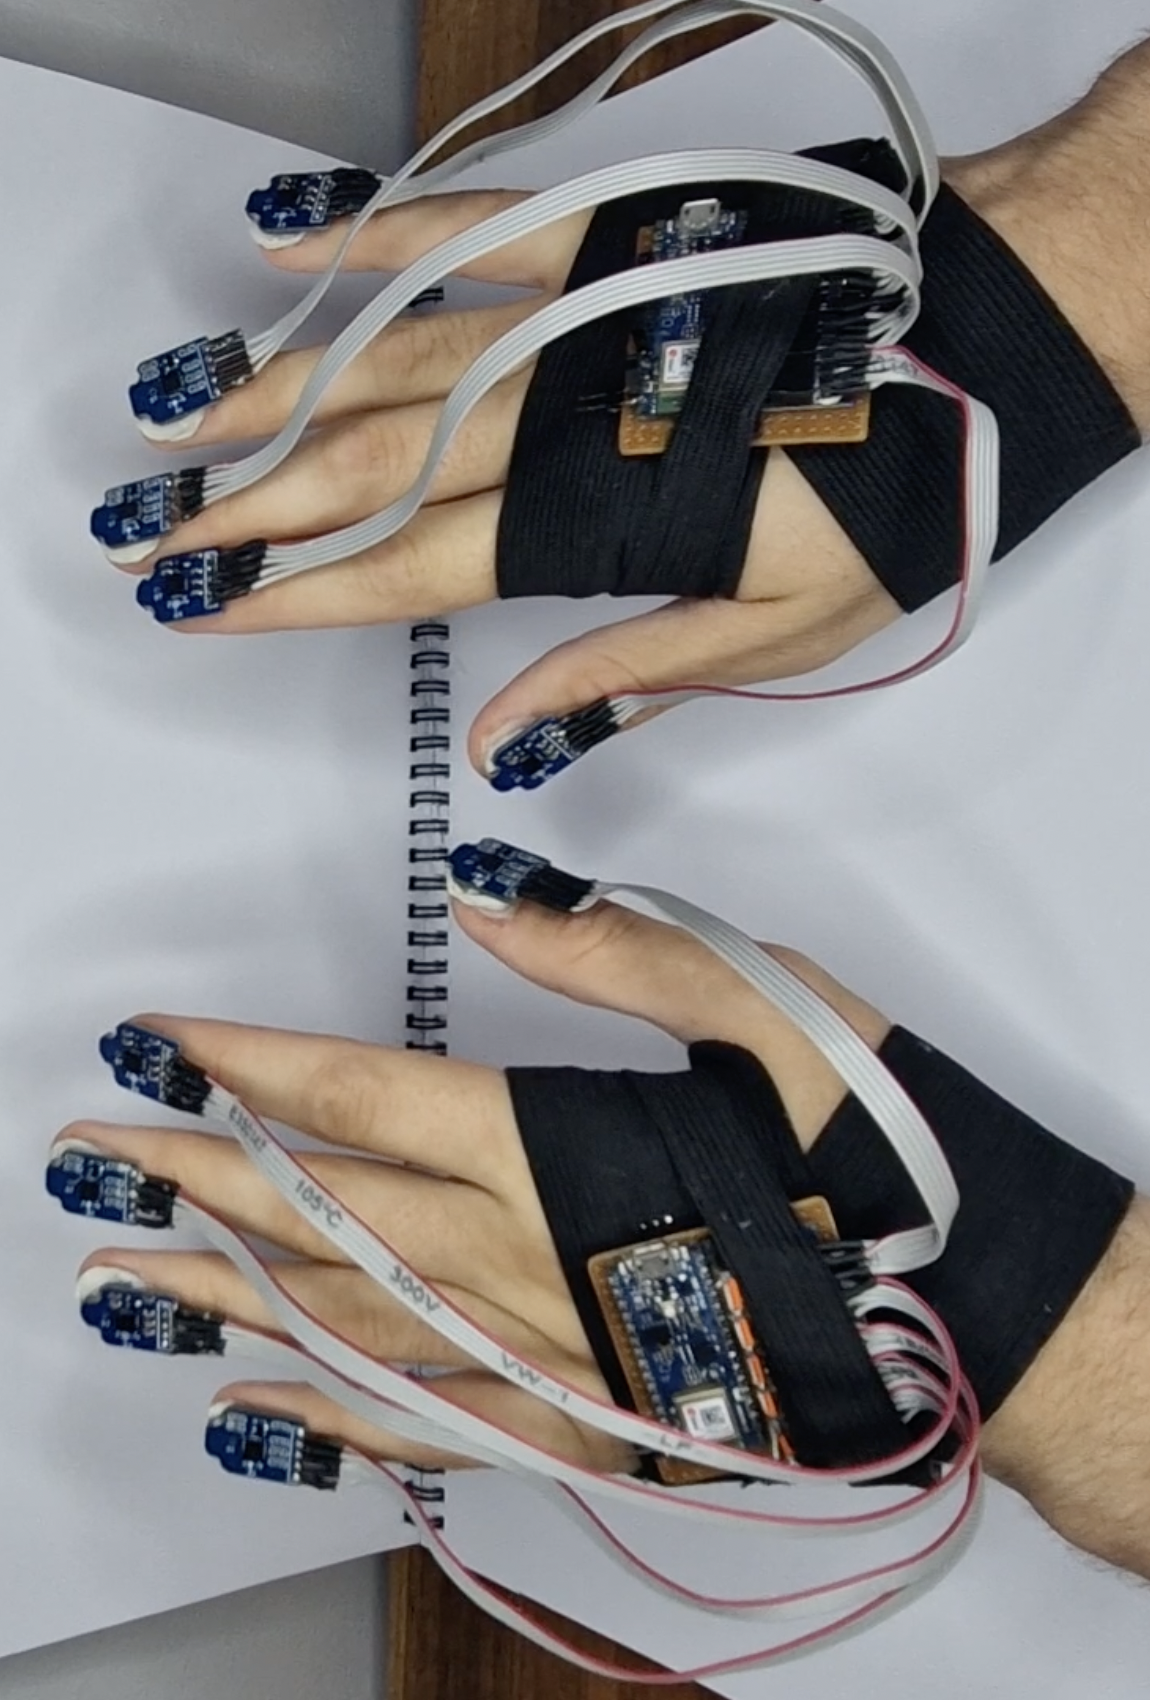
\includegraphics[height=5.5cm, angle=270]{imgs/glove}}}

\begin{document}
\begin{frame}
  \maketitle
\end{frame}

\section{Overview}
\begin{frame}
    \frametitle{A video demonstration}
    \begin{figure}[h]
        \centering
        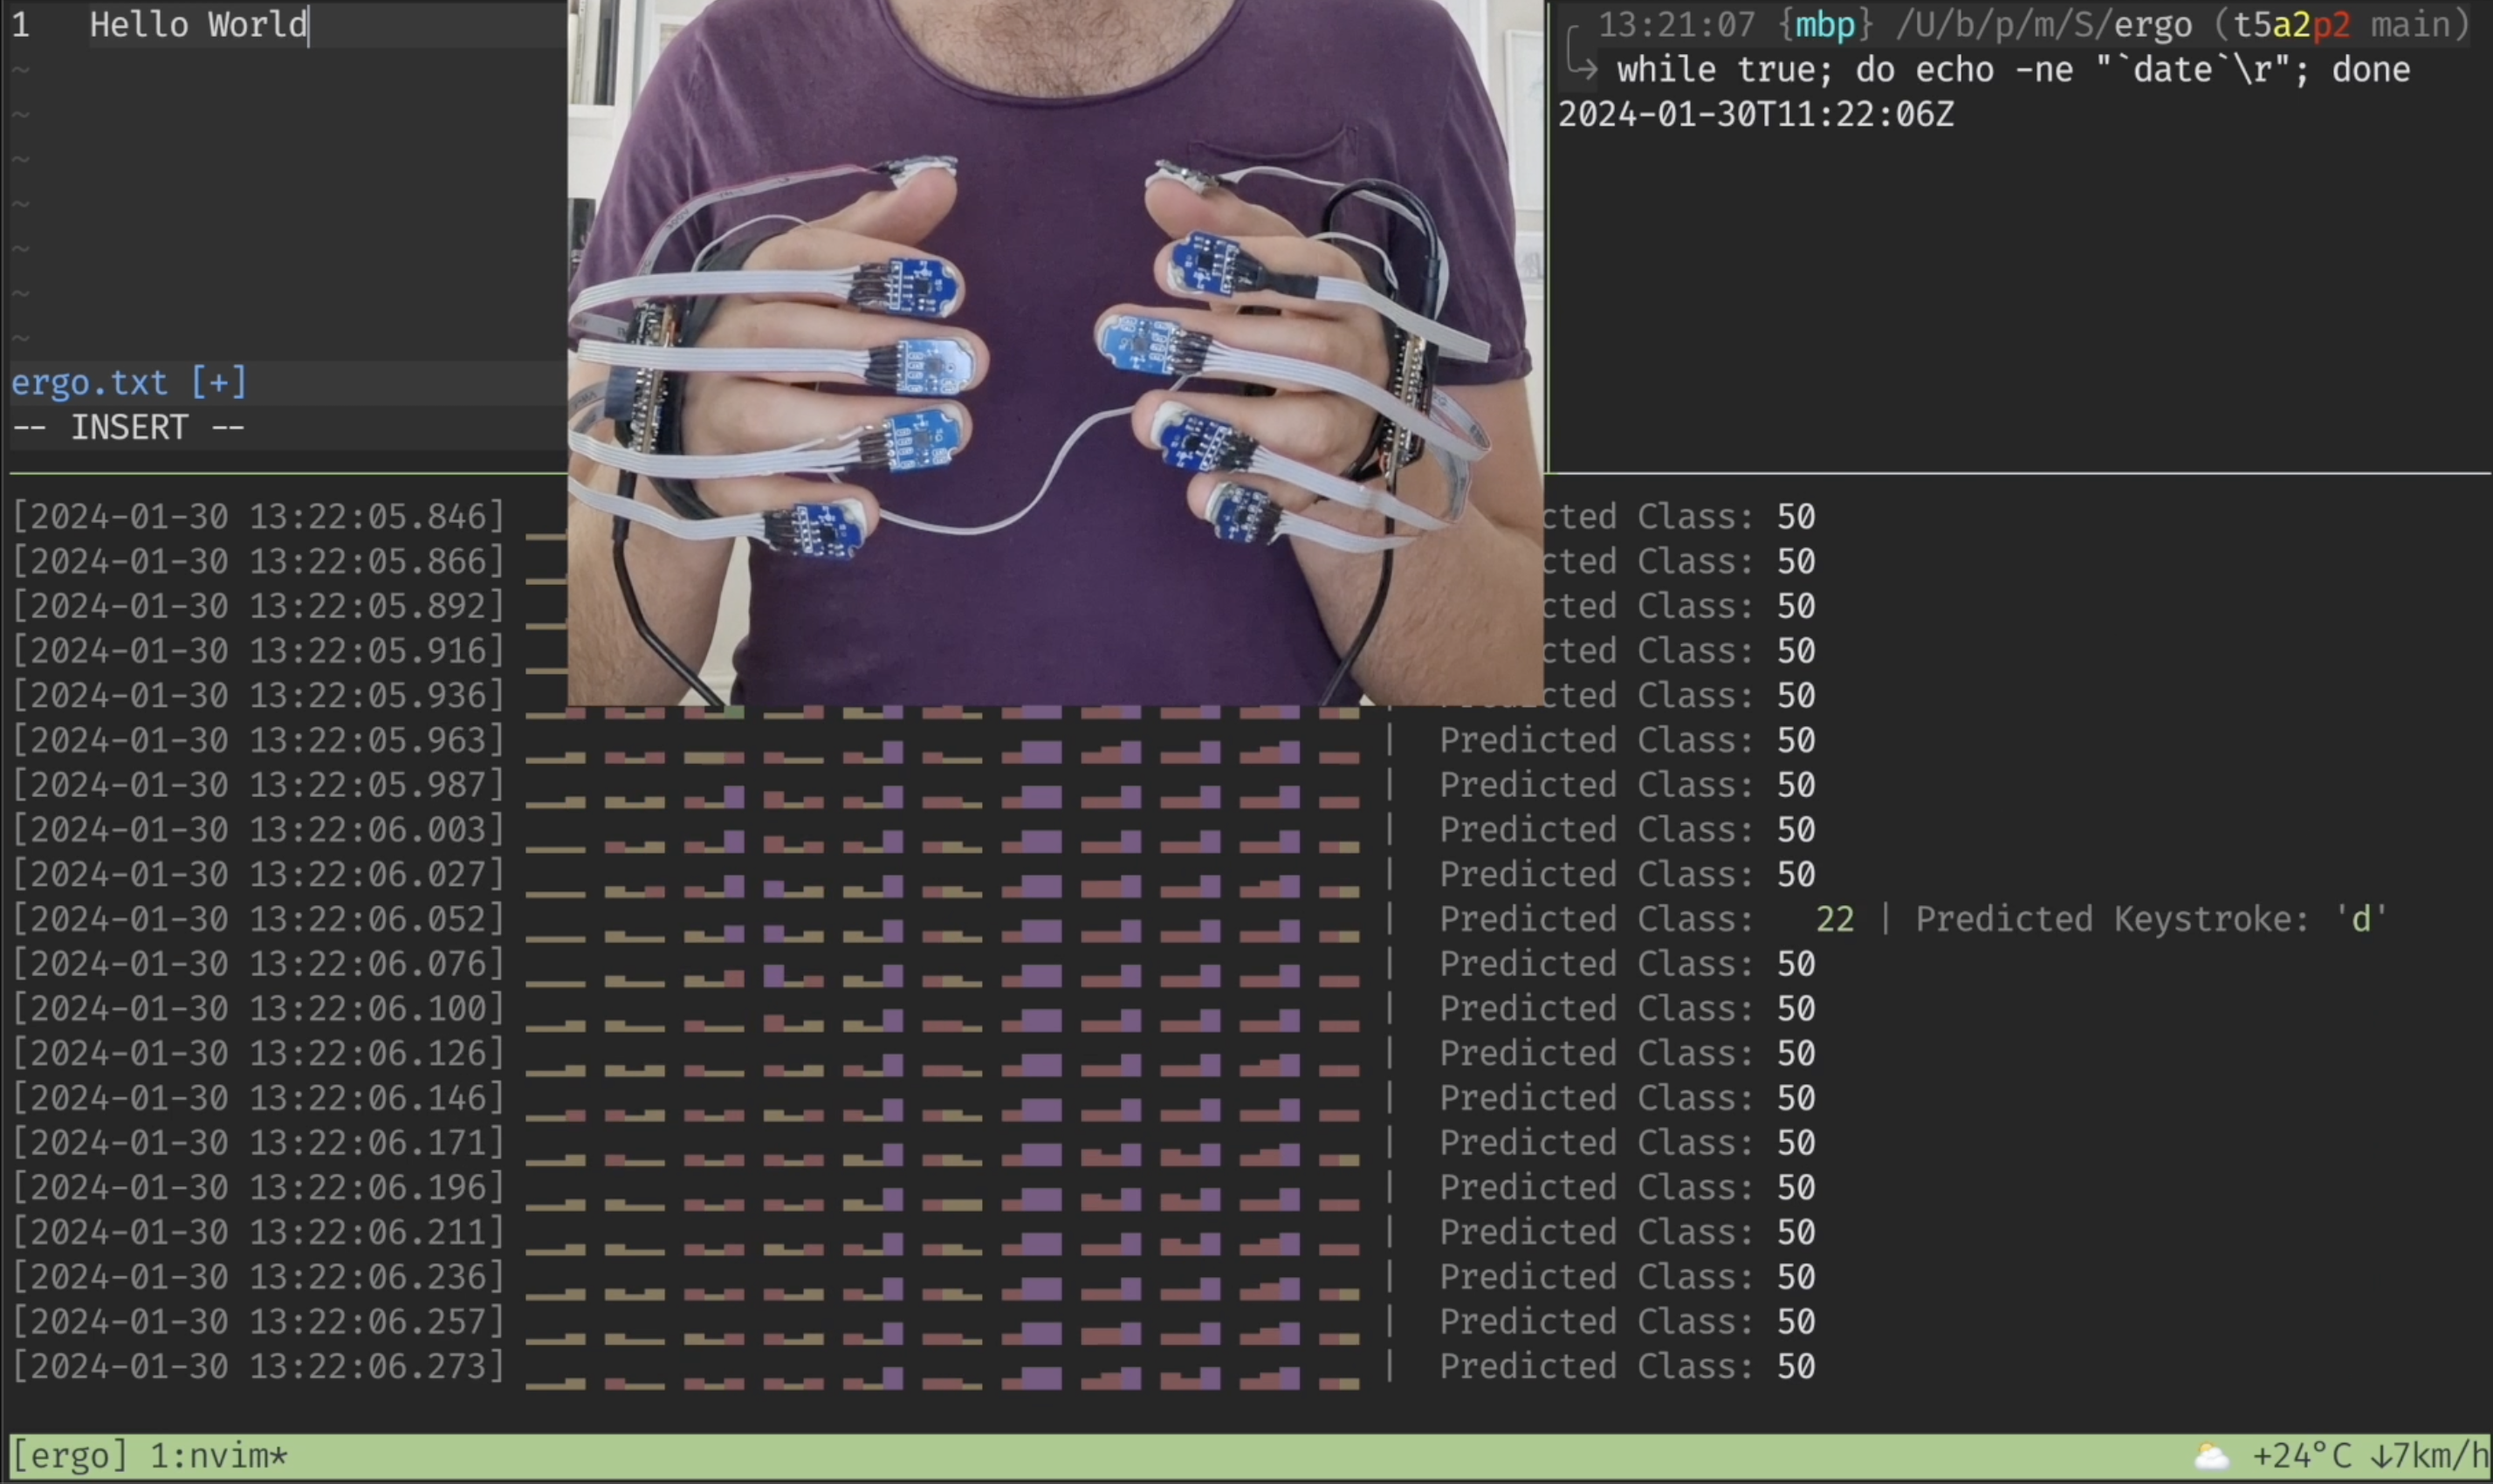
\includegraphics[width=0.9\textwidth]{imgs/video_thumbnail.png}
    \end{figure}
    \emph{Ergo} in a nutshell:
    \begin{enumerate}
        \item Similar to a glove in form-factor
        \item Sensors measure fingertip acceleration
        \item Acceleration measurements are classified into gestures
        \item Gestures are mapped to keystrokes
        \item Keystrokes are sent to the operating system
    \end{enumerate}
\end{frame}

\section{Introduction}
\begin{frame}
    \frametitle{Introduction}
    \framesubtitle{Research questions}
    \centering
    1. Evaluate hardware performance
\end{frame}

\begin{frame}
    \frametitle{Introduction}
    \framesubtitle{Research questions}
    \centering
    2. Compare algorithm performance
\end{frame}

\begin{frame}
    \frametitle{Introduction}
    \framesubtitle{Research questions}
    \centering
    3. Extract gestures from background noise
\end{frame}

\begin{frame}
    \frametitle{Introduction}
    \framesubtitle{Research questions}
    \centering
    4. Assess impact of noise on performance
\end{frame}

\begin{frame}
    \frametitle{Introduction}
    \framesubtitle{Research questions}
    \centering
    5. Assess classification speed
\end{frame}

\begin{frame}
    \frametitle{Introduction}
    \framesubtitle{Open Code \& Open Data}
    \begin{itemize}
        \item All code is on
            GitHub\footnote{https://github.com/beyarkay/masters‐code}.
        \item The source code for the thesis (and this presentation) is also on
            GitHub\footnote{https://github.com/beyarkay/masters‐thesis}.
        \item The dataset is on
            Zenodo\footnote{https://zenodo.org/records/10209419}.
        \item The video played at the beginning of the presentation is
            available on
            YouTube\footnote{https://www.youtube.com/watch?v=vFsaH1TqNWo}.
    \end{itemize}
\end{frame}

\section{Background}

\begin{frame}
    \frametitle{Background}
    \framesubtitle{Feed-Forward Neural Networks (FFNNs)}
    \begin{figure}
        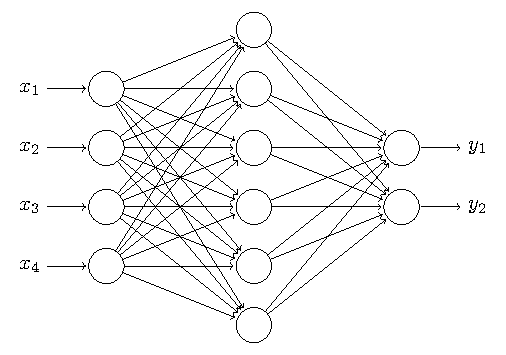
\includegraphics{imgs/neural_network.pdf}
    \end{figure}
\end{frame}

\begin{frame}
    \frametitle{Background}
    \framesubtitle{Support Vector Machines (SVMs)}
    \begin{figure}
        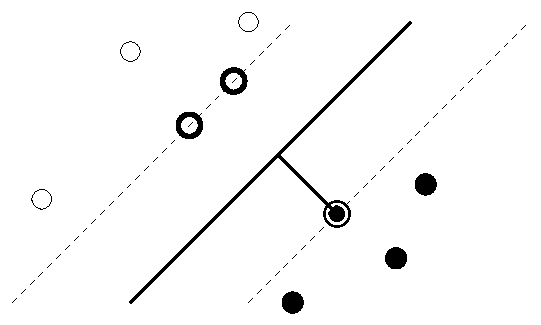
\includegraphics{imgs/support_vector_machines.pdf}
    \end{figure}
\end{frame}

\begin{frame}
    \frametitle{Background}
    \framesubtitle{Hidden Markov Models (HMMs)}
    \begin{figure}
        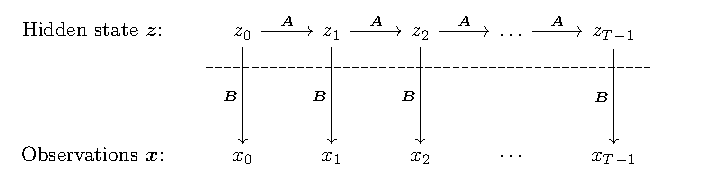
\includegraphics[width=\textwidth]{imgs/hidden_markov_model.pdf}
    \end{figure}
\end{frame}

\begin{frame}
    \frametitle{Background}
    \framesubtitle{Cumulative Sum (CuSUM)}
    \begin{figure}
        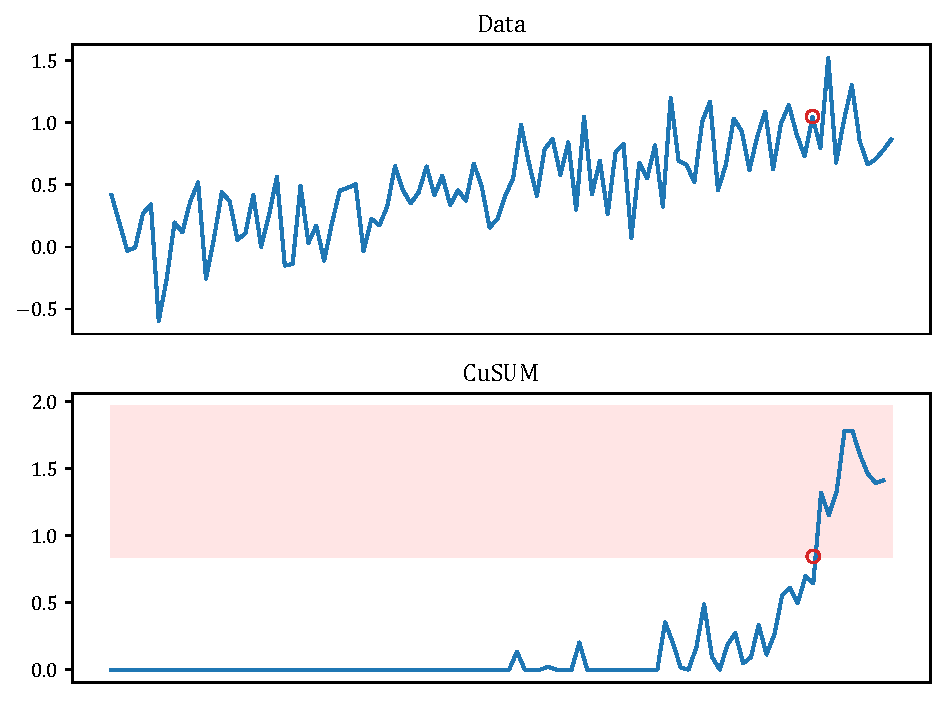
\includegraphics[width=\textwidth]{imgs/cusum.pdf}
    \end{figure}
\end{frame}


\begin{frame}
    \frametitle{Background}
    \framesubtitle{Confusion Matrices}
    \begin{figure}
        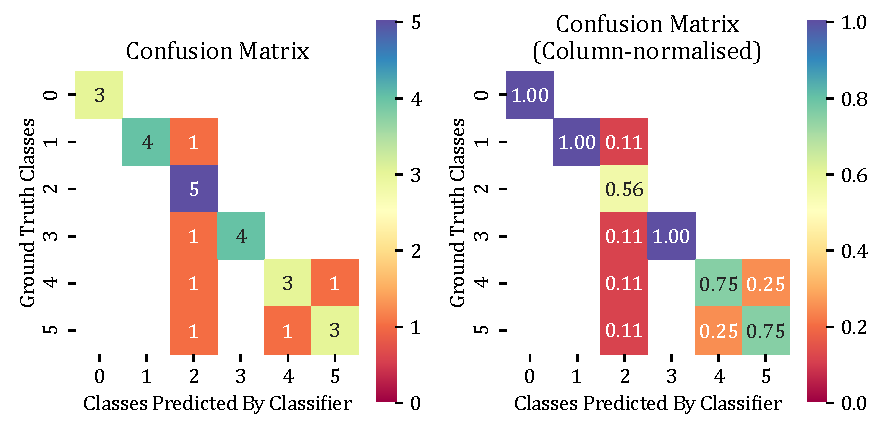
\includegraphics[width=\textwidth]{imgs/conf_mats.pdf}
    \end{figure}
\end{frame}

\begin{frame}
    \frametitle{Background}
    \framesubtitle{Precision and Recall}
    \begin{figure}
        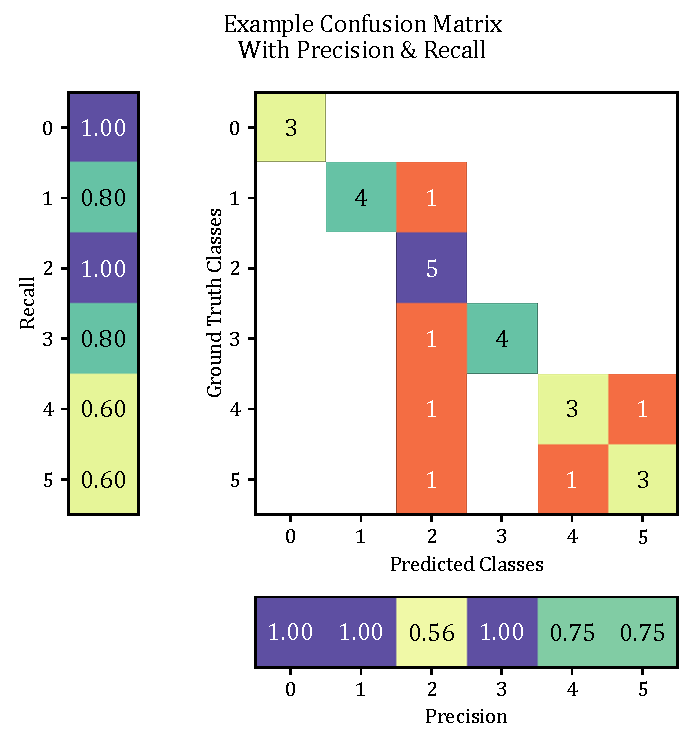
\includegraphics[width=0.75\textwidth]{imgs/conf_mat_prec_recall.pdf}
    \end{figure}
\end{frame}

\begin{frame}
    \frametitle{Background}
    \framesubtitle{$F_1$-score}
    $$ F_{1} = 2 \cdot \frac{ \text{Precision} \cdot \text{Recall} }{ \text{Precision} + \text{Recall} } $$
    \begin{figure}
        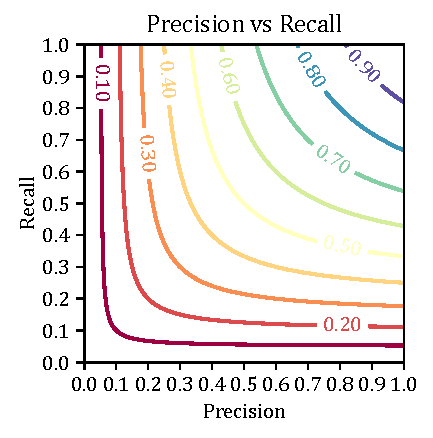
\includegraphics[width=0.6\textwidth]{imgs/04_precision_recall_f1.pdf}
    \end{figure}
\end{frame}

\section{Literature Review}
\begin{frame}
    \frametitle{Literature Review}
    \framesubtitle{Seminal work}
    \begin{columns}
        \begin{column}{.5\textwidth}
            \begin{figure}
                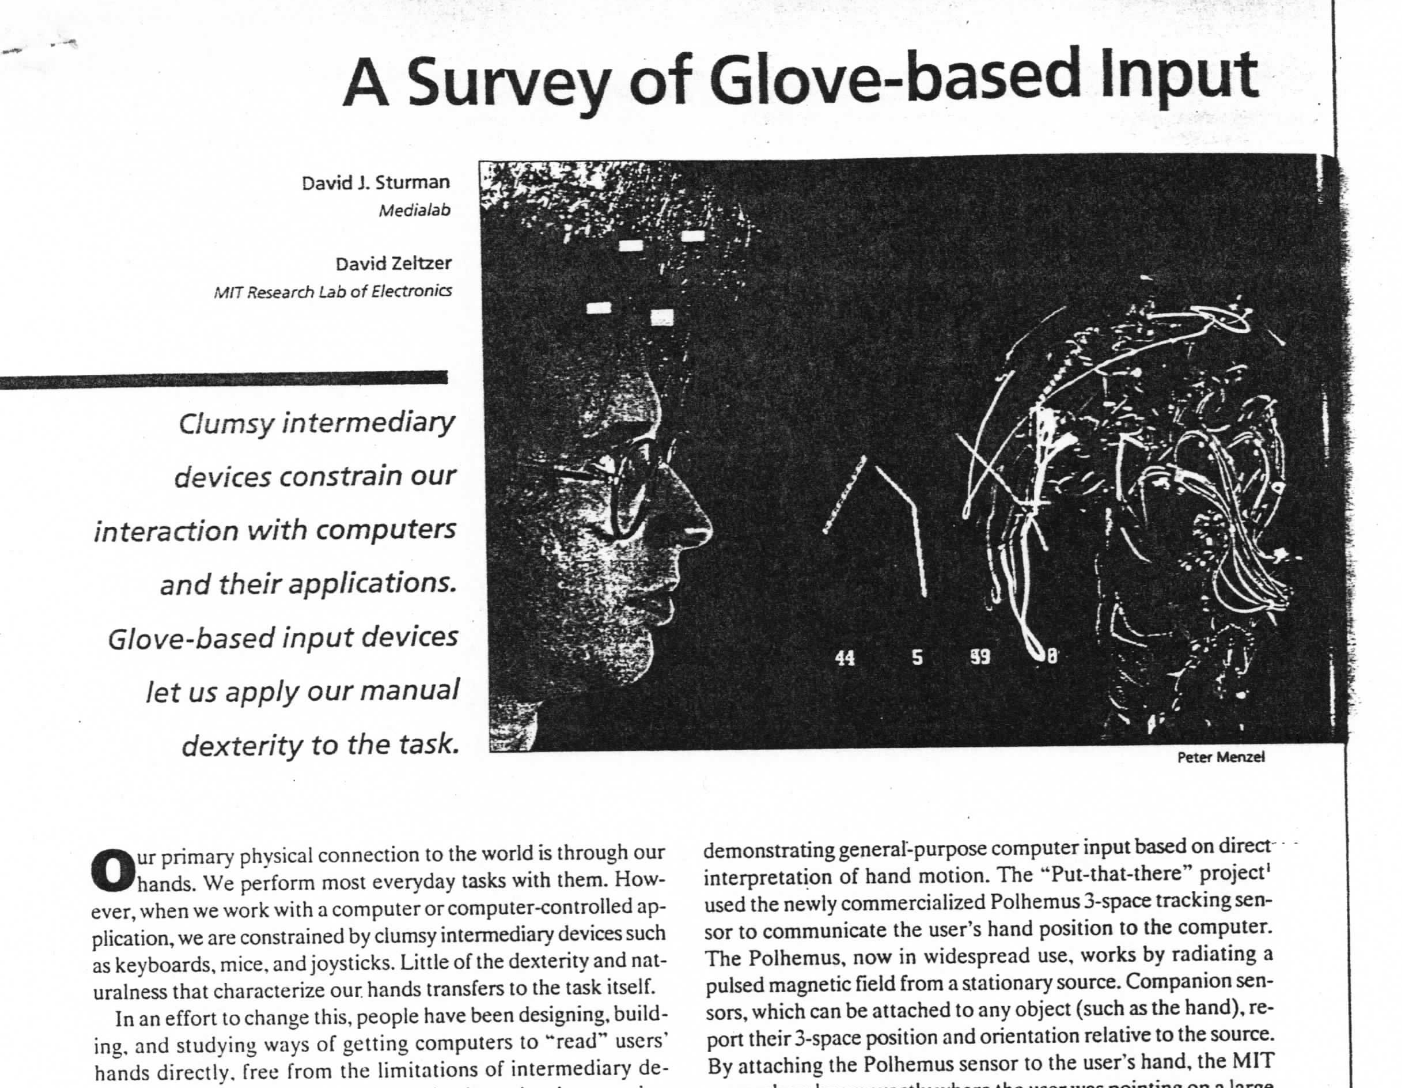
\includegraphics[width=0.9\textwidth]{imgs/sturman.png}
                \caption{Sturman and Zeltzer (1994) discussed hardware systems}
            \end{figure}
        \end{column}
        \begin{column}{.5\textwidth}
            \begin{figure}
                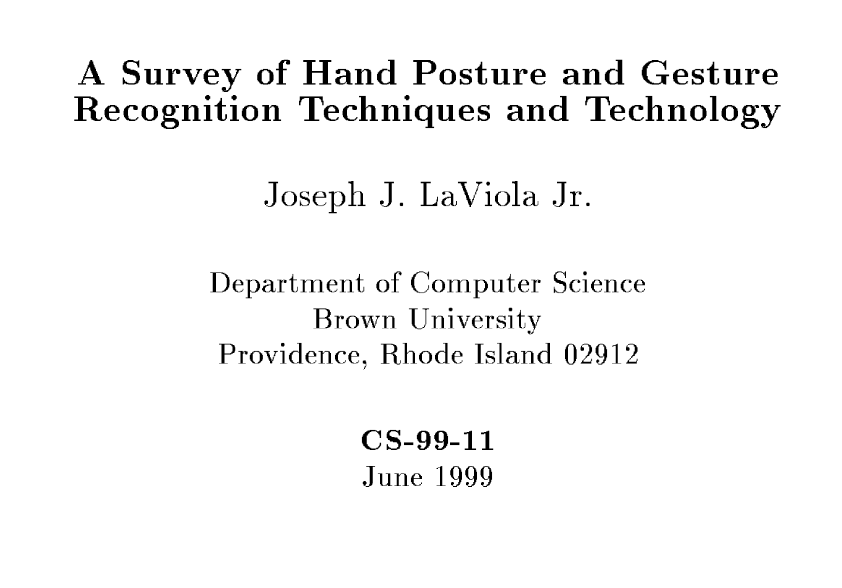
\includegraphics[width=0.9\textwidth]{imgs/laviola.png}
                \caption{LaViola (1999) discussed models and techniques}
            \end{figure}
        \end{column}
    \end{columns}
\end{frame}

\begin{frame}
    \frametitle{Literature Review}
    \framesubtitle{Technologies Used Over Time}
    \begin{figure}
        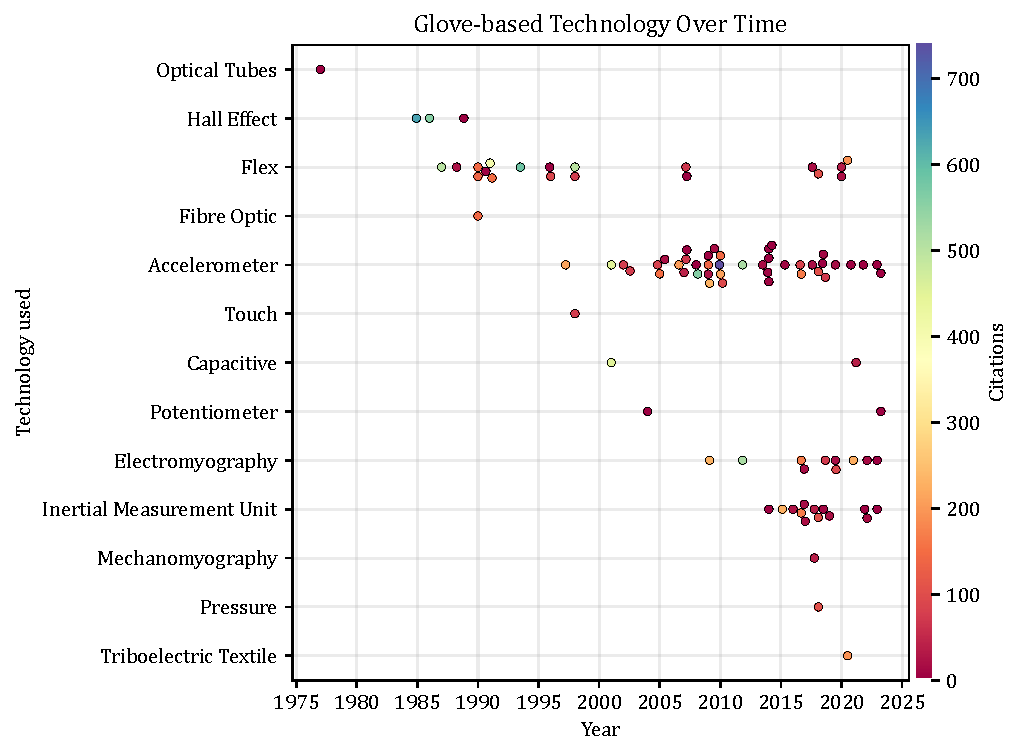
\includegraphics[width=0.9\textwidth]{imgs/03_tech_for_gloves.pdf}
    \end{figure}
\end{frame}

\begin{frame}
    \frametitle{Literature Review}
    \framesubtitle{Number of Classes Over Time}
    \begin{figure}
        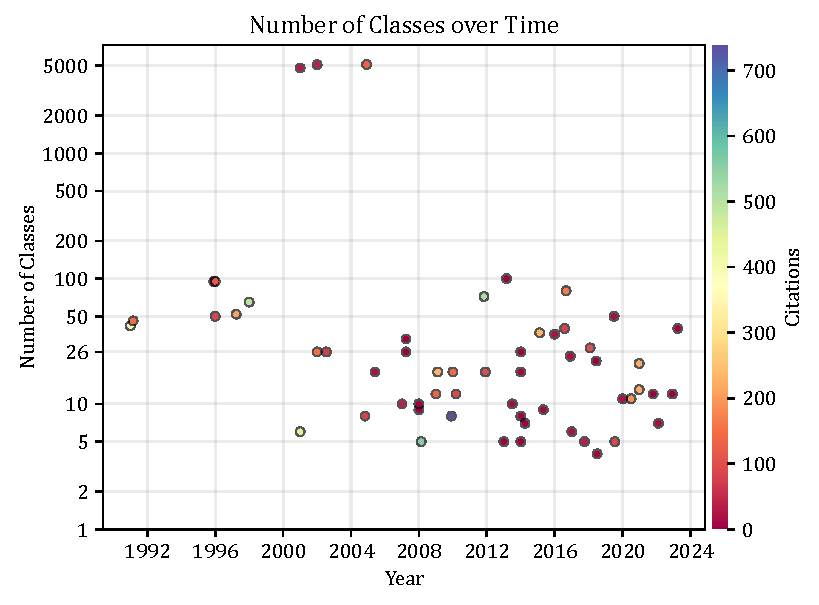
\includegraphics[width=0.9\textwidth]{imgs/03_date_vs_nclasses.pdf}
    \end{figure}
\end{frame}

\begin{frame}
    \frametitle{Literature Review}
    \framesubtitle{Algorithms Used Over Time}
    \begin{figure}
        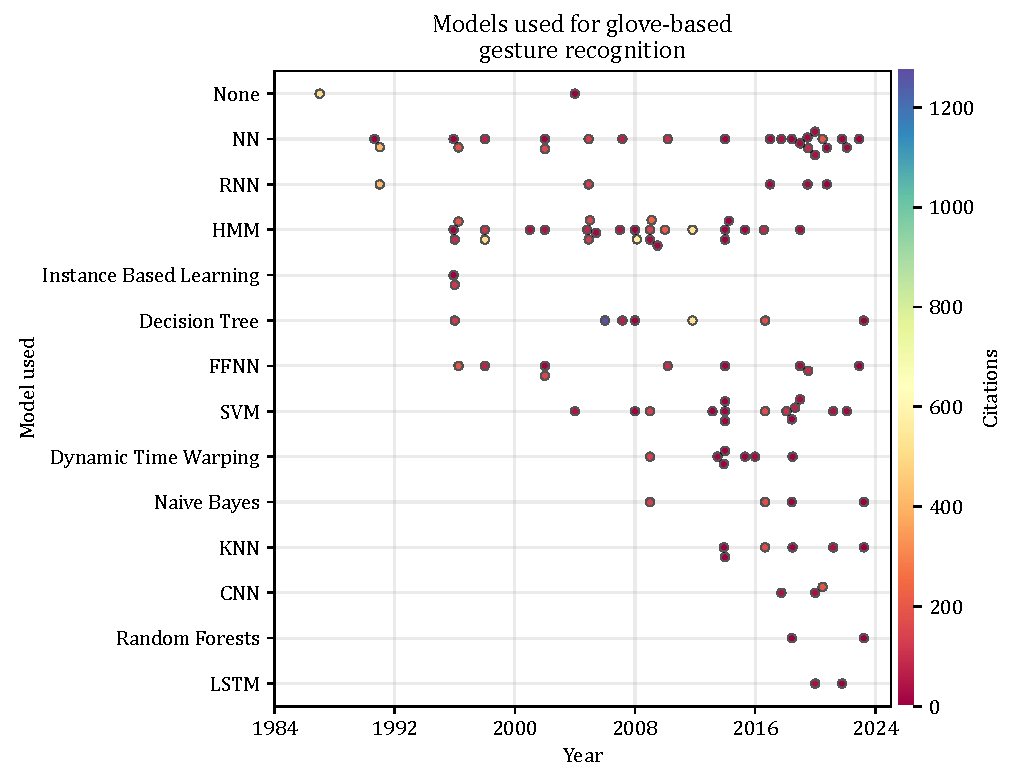
\includegraphics[width=0.9\textwidth]{imgs/03_models_glove_based.pdf}
    \end{figure}
\end{frame}

\begin{frame}
    \frametitle{Literature Review}
    \framesubtitle{Gesture Fidelity Over Time}
    \begin{figure}
        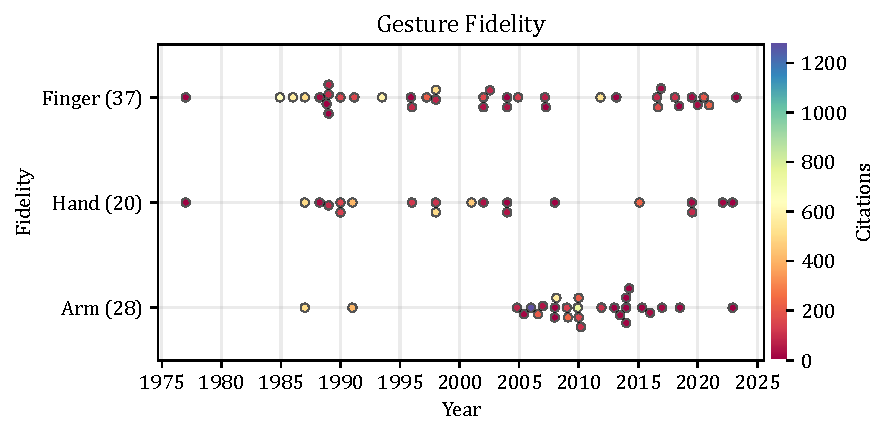
\includegraphics[width=0.9\textwidth]{imgs/03_fidelity_for_gloves.pdf}
    \end{figure}
\end{frame}

\begin{frame}
    \frametitle{Literature Review}
    \framesubtitle{Explicit/Implicit Segmentation Over Time}
    \begin{figure}
        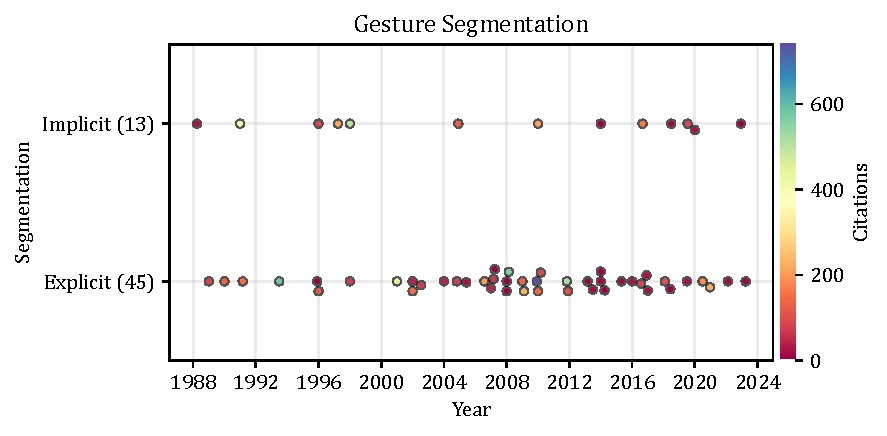
\includegraphics[width=0.9\textwidth]{imgs/03_segmentation_for_gloves.pdf}
    \end{figure}
\end{frame}

\section{Methodology}
\begin{frame}
    \frametitle{Methodology}
    \framesubtitle{Circuit Diagram of \emph{Ergo}}
    \begin{figure}[h]
        \centering
        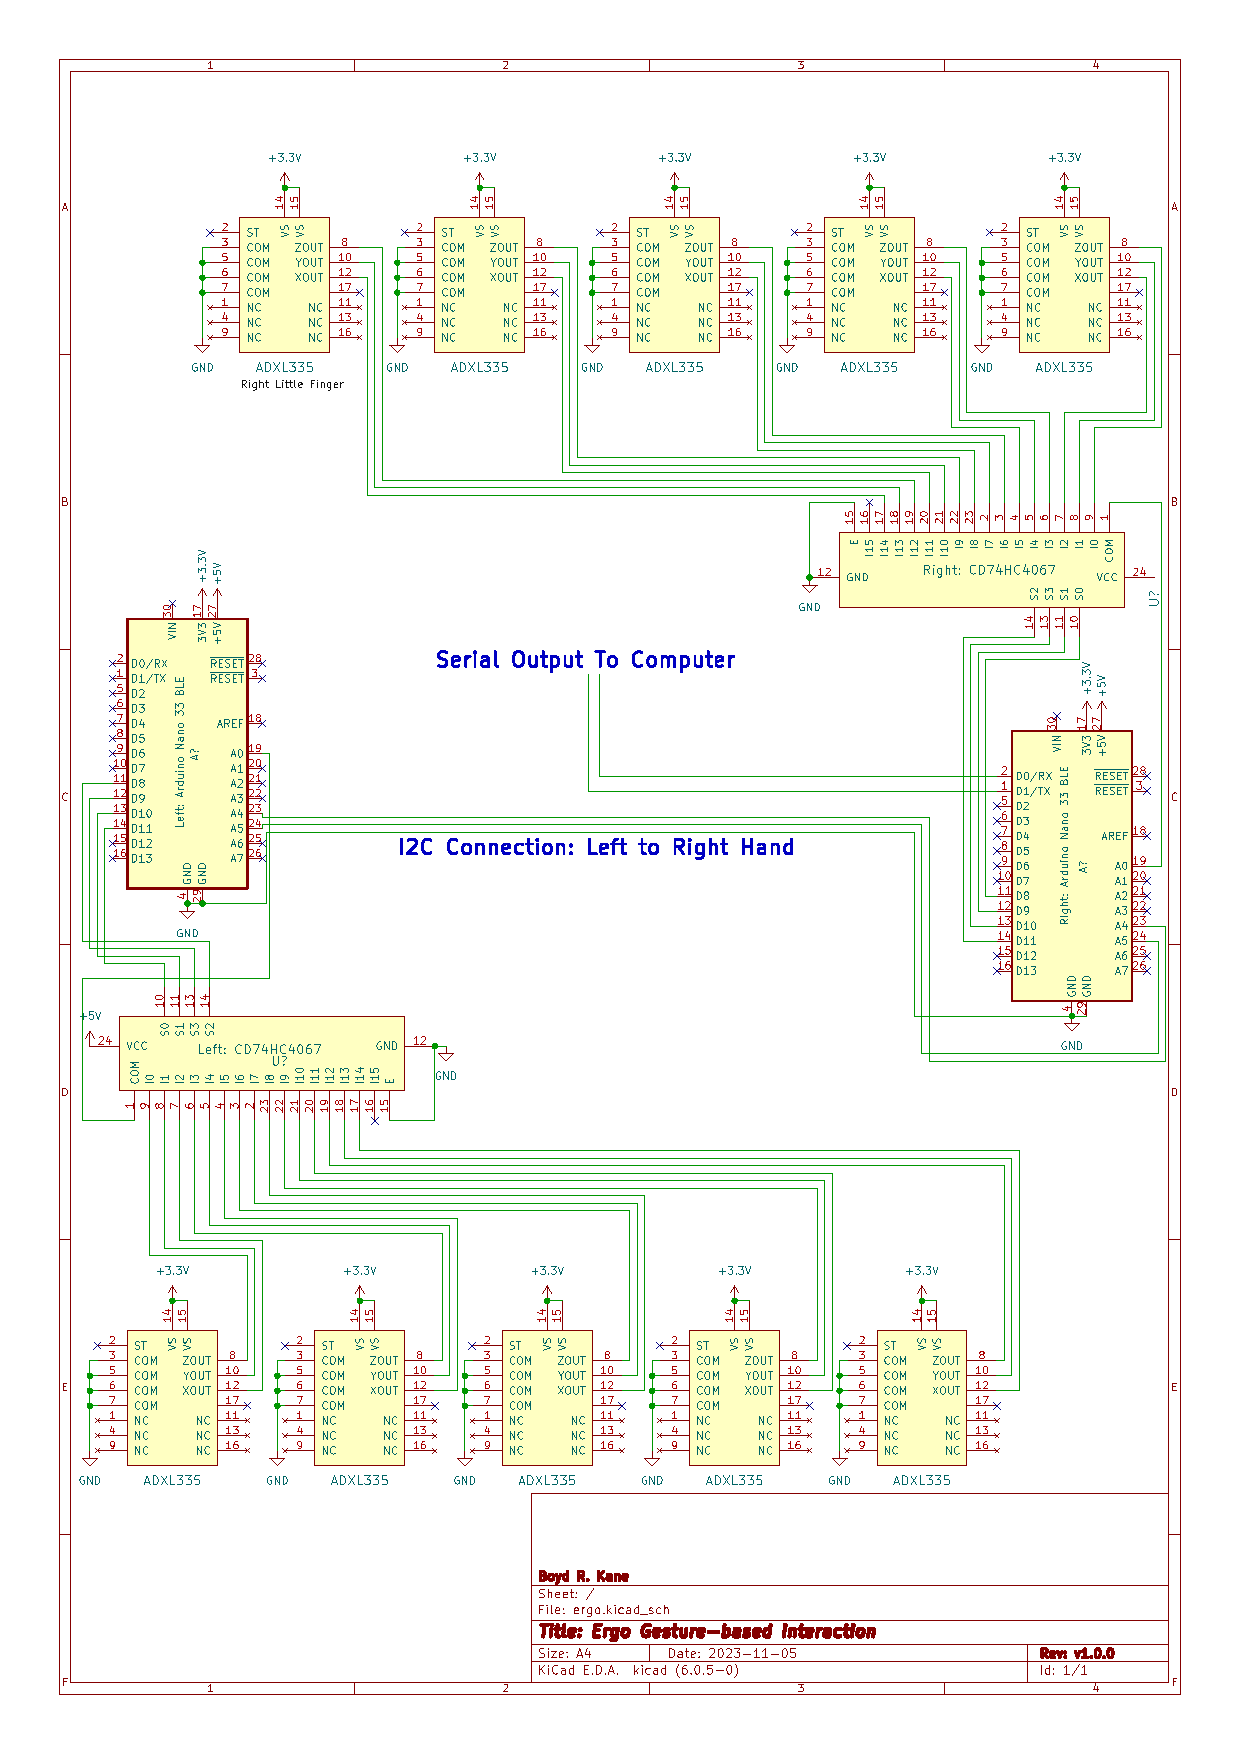
\includegraphics[height=0.8\textheight]{imgs/ergo_schematic.pdf}
    \end{figure}
\end{frame}

\begin{frame}
    \frametitle{Methodology}
    \framesubtitle{Gestures to Keystrokes}
    \begin{figure}[h]
        \centering
        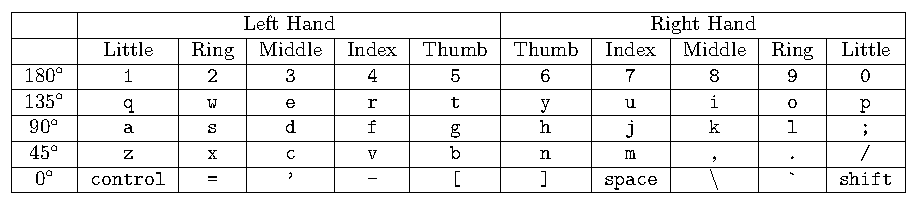
\includegraphics[width=\textwidth]{imgs/gesture_to_keystrokes.pdf}
        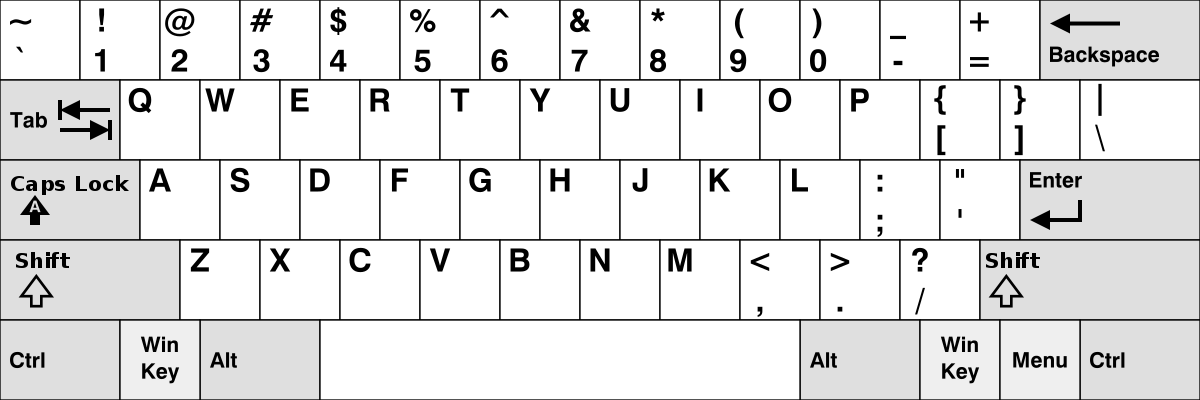
\includegraphics[width=\textwidth]{imgs/qwerty_keyboard.png}
        \caption{QWERTY keyboard image from Wikimedia Commons, licensed CC BY-SA 3.0}
    \end{figure}
\end{frame}

\begin{frame}
    \frametitle{Methodology}
    \framesubtitle{Gesture Indices}
    \begin{figure}[h]
        \centering
        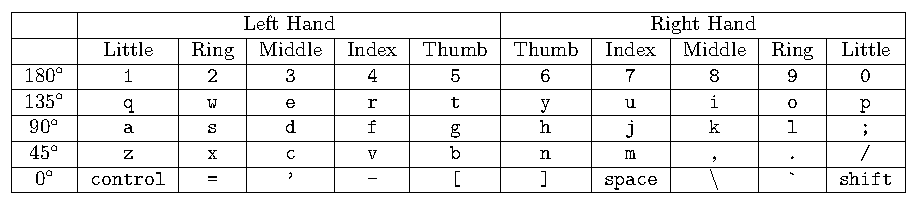
\includegraphics[width=\textwidth]{imgs/gesture_to_keystrokes.pdf}
        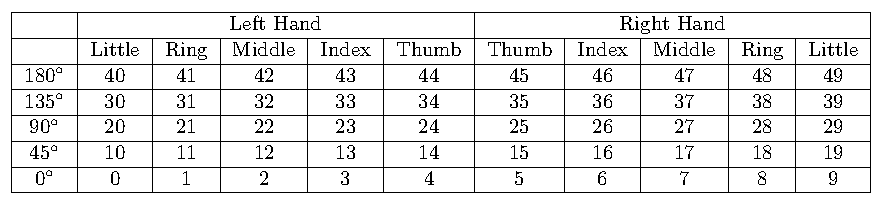
\includegraphics[width=\textwidth]{imgs/gesture_to_indices.pdf}
    \end{figure}
\end{frame}

\begin{frame}
    \frametitle{Methodology}
    \framesubtitle{Class 50 - Background Noise}

    \begin{figure}[h]
        \centering
        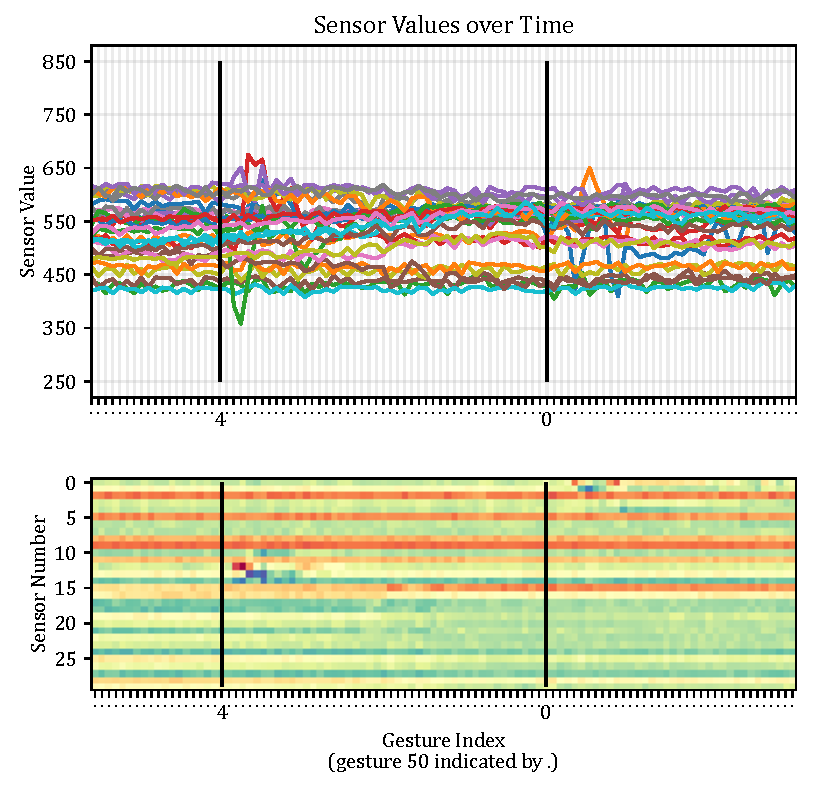
\includegraphics[width=0.8\textwidth]{imgs/04_sensors_over_time.pdf}
    \end{figure}
\end{frame}

\begin{frame}
    \frametitle{Methodology}
    \framesubtitle{Data windowing}
    \begin{figure}[h]
        \centering
        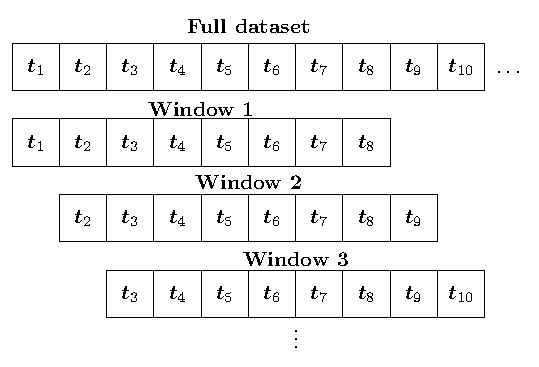
\includegraphics[width=\textwidth]{imgs/windowing_tikz.pdf}
    \end{figure}
\end{frame}

\begin{frame}
    \frametitle{Methodology}
    \centering{Hierarchical Feed-Forward Neural Networks}
\end{frame}

\section{Results}
\begin{frame}
    \frametitle{Results}
    \framesubtitle{Cumulative Sum}
    \begin{figure}[h]
        \centering
        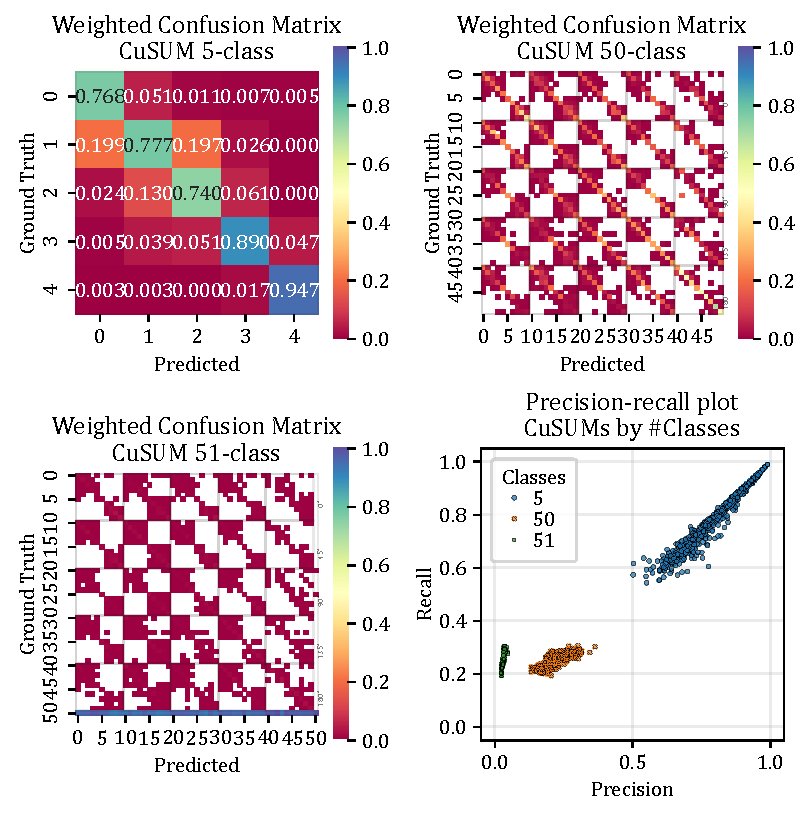
\includegraphics[width=0.8\textwidth]{imgs/05_mean_conf_mat_cusum.pdf}
    \end{figure}
\end{frame}

\begin{frame}
    \frametitle{Results}
    \framesubtitle{Hidden Markov Models}
    \begin{figure}[h]
        \centering
        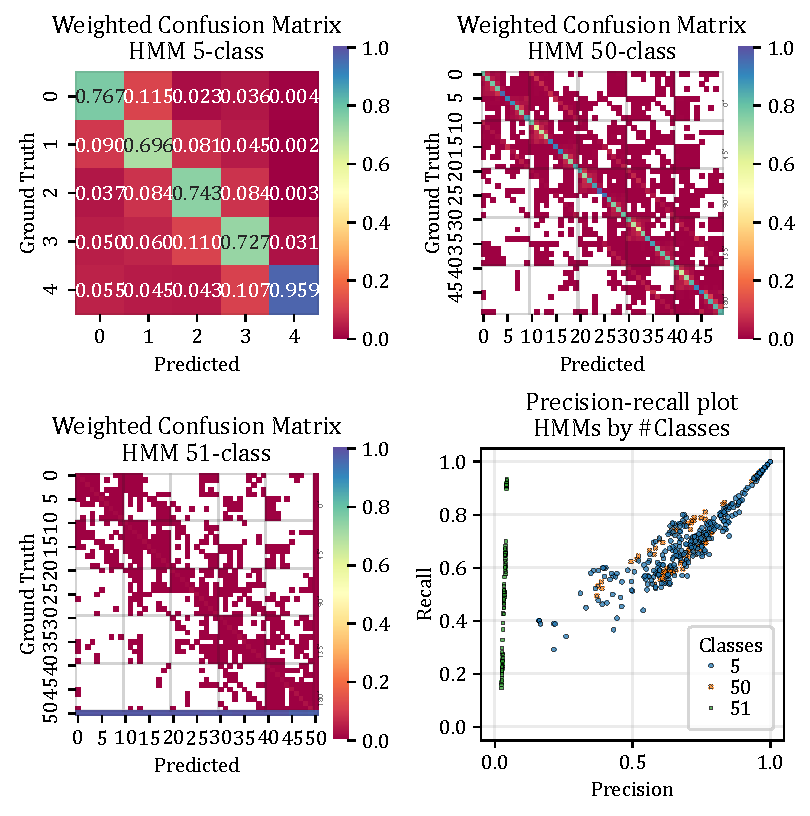
\includegraphics[width=0.8\textwidth]{imgs/05_mean_conf_mat_hmm.pdf}
    \end{figure}
\end{frame}

\begin{frame}
    \frametitle{Results}
    \framesubtitle{Support Vector Machines}
    \begin{figure}[h]
        \centering
        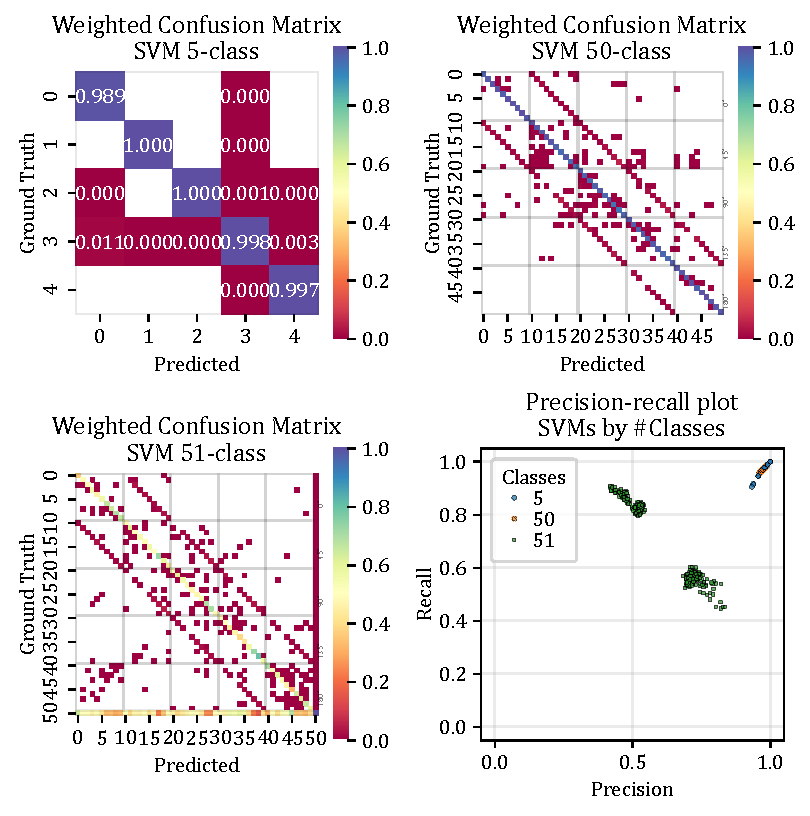
\includegraphics[width=0.8\textwidth]{imgs/05_mean_conf_mat_svm.pdf}
    \end{figure}
\end{frame}

\begin{frame}
    \frametitle{Results}
    \framesubtitle{Feed-forward Neural Networks}
    \begin{figure}[h]
        \centering
        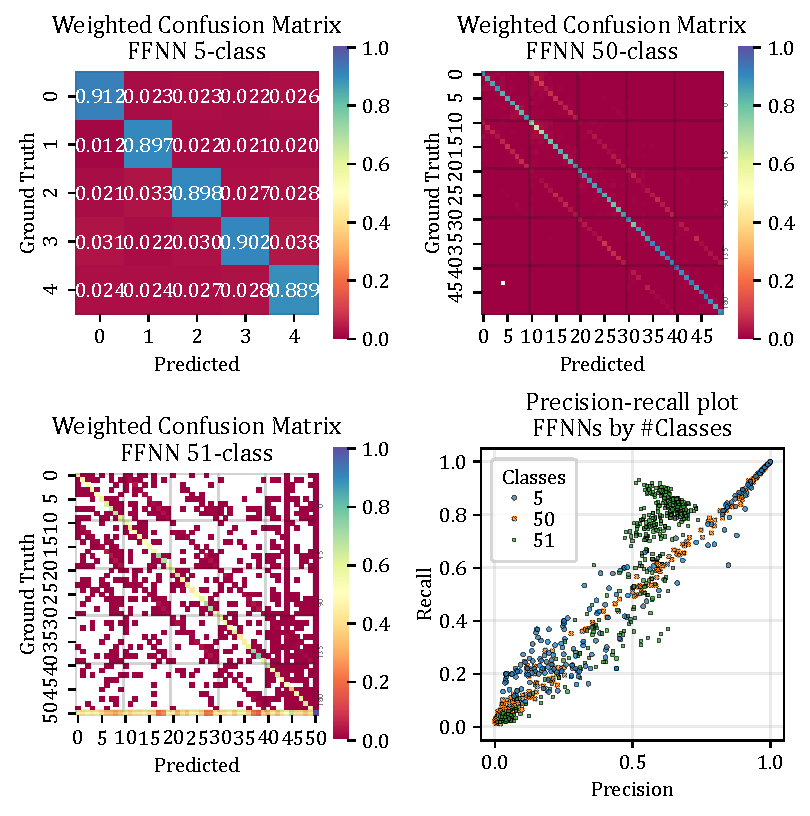
\includegraphics[width=0.8\textwidth]{imgs/05_mean_conf_mat_ffnn.pdf}
    \end{figure}
\end{frame}


\begin{frame}
    \frametitle{Results}
    \framesubtitle{Hierarchical Feed-forward Neural Networks}
    \begin{figure}[h]
        \centering
        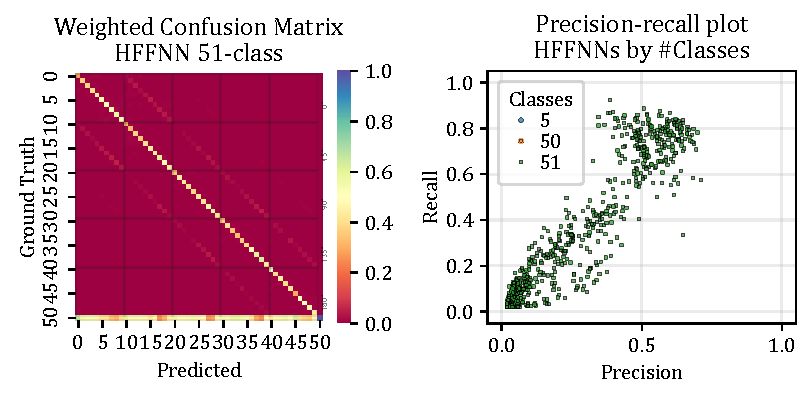
\includegraphics[width=0.9\textwidth]{imgs/05_mean_conf_mat_hffnn.pdf}
    \end{figure}
\end{frame}

\begin{frame}
    \frametitle{Results}
    \framesubtitle{Comparison Between The Models}
    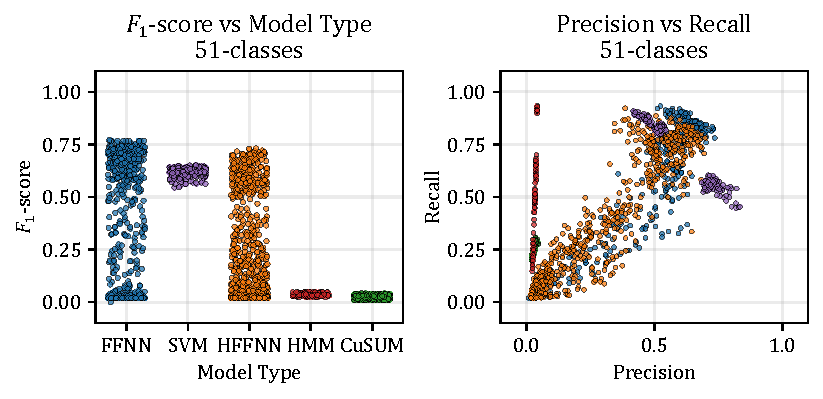
\includegraphics[width=\textwidth]{imgs/05_precision_recall_51_classes.pdf}
\end{frame}

\begin{frame}
    \frametitle{Results}
    \framesubtitle{Real-world typing}
    \centering
    \texttt{the quick brown fox jumped over the lazy dog}
    \begin{figure}[h]
        \centering
        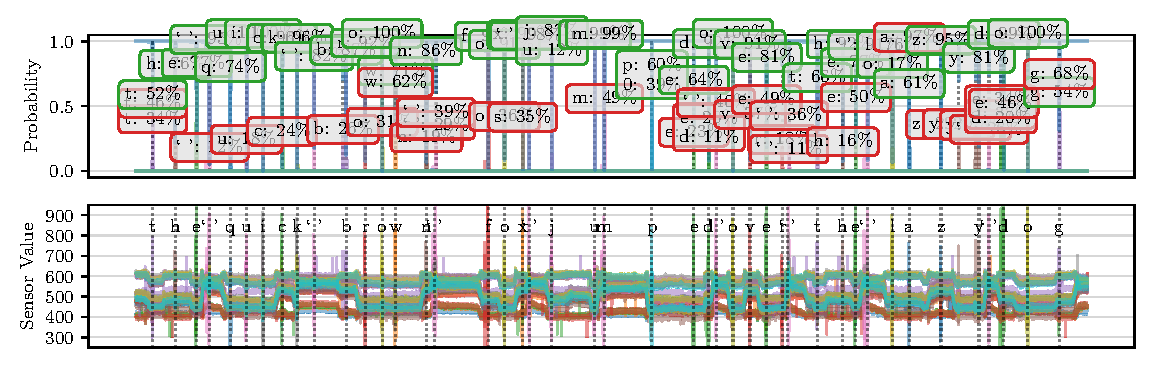
\includegraphics[width=\textwidth]{imgs/05_pred_plot_0000_to_9420_full_text.pdf}
    \end{figure}
\end{frame}

\begin{frame}
    \frametitle{Results}
    \framesubtitle{Real-world typing}
    \centering
    \texttt{quick }
    \begin{figure}[h]
        \centering
        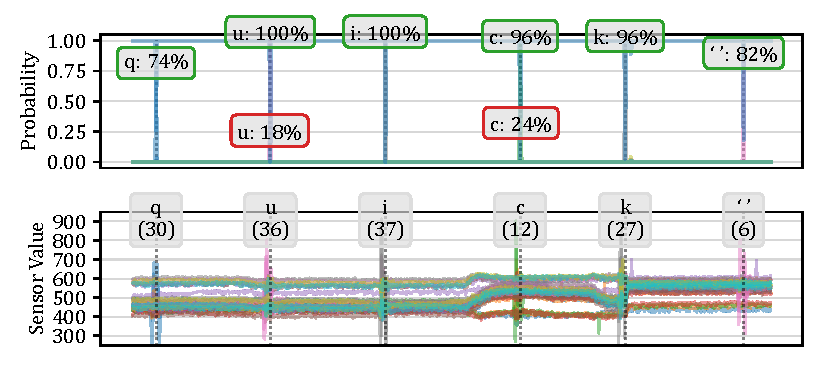
\includegraphics[width=\textwidth]{imgs/05_pred_plot_0900_to_1800_quick.pdf}
    \end{figure}
\end{frame}

\begin{frame}
    \frametitle{Results}
    \framesubtitle{Inference Speed}
    \begin{figure}[h]
        \centering
        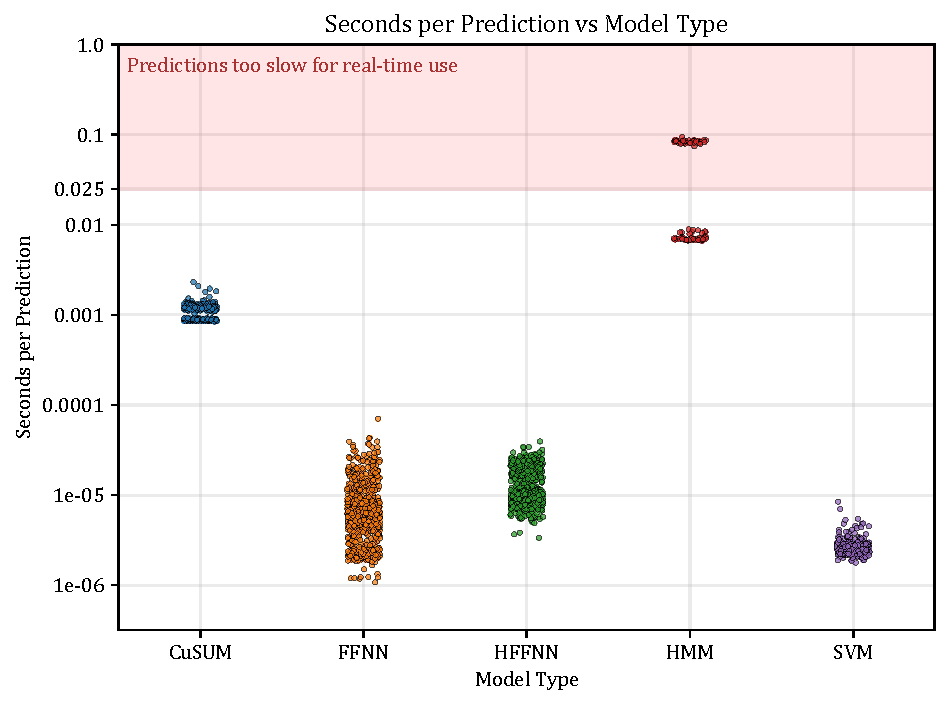
\includegraphics[width=\textwidth]{imgs/inference_time_per_obs_per_model.pdf}
    \end{figure}
\end{frame}

\section{Conclusion}
\begin{frame}
    \frametitle{Conclusion}
    Research Questions:
    \begin{enumerate}
        \item Evaluate hardware performance
        \item Compare algorithm performance
        \item Extract gestures from background noise
        \item Assess impact of noise on performance
        \item Assess classification speed
    \end{enumerate}
\end{frame}

\section{Questions}
\begin{frame}
    \centering
    Questions?
\end{frame}


\end{document}
